% Options for packages loaded elsewhere
\PassOptionsToPackage{unicode}{hyperref}
\PassOptionsToPackage{hyphens}{url}
%
\documentclass[
  11pt,
  ignorenonframetext,
]{beamer}
\usepackage{pgfpages}
\setbeamertemplate{caption}[numbered]
\setbeamertemplate{caption label separator}{: }
\setbeamercolor{caption name}{fg=normal text.fg}
\beamertemplatenavigationsymbolsempty
% Prevent slide breaks in the middle of a paragraph
\widowpenalties 1 10000
\raggedbottom
\setbeamertemplate{part page}{
  \centering
  \begin{beamercolorbox}[sep=16pt,center]{part title}
    \usebeamerfont{part title}\insertpart\par
  \end{beamercolorbox}
}
\setbeamertemplate{section page}{
  \centering
  \begin{beamercolorbox}[sep=12pt,center]{part title}
    \usebeamerfont{section title}\insertsection\par
  \end{beamercolorbox}
}
\setbeamertemplate{subsection page}{
  \centering
  \begin{beamercolorbox}[sep=8pt,center]{part title}
    \usebeamerfont{subsection title}\insertsubsection\par
  \end{beamercolorbox}
}
\AtBeginPart{
  \frame{\partpage}
}
\AtBeginSection{
  \ifbibliography
  \else
    \frame{\sectionpage}
  \fi
}
\AtBeginSubsection{
  \frame{\subsectionpage}
}

\usepackage{amsmath,amssymb}
\usepackage{iftex}
\ifPDFTeX
  \usepackage[T1]{fontenc}
  \usepackage[utf8]{inputenc}
  \usepackage{textcomp} % provide euro and other symbols
\else % if luatex or xetex
  \usepackage{unicode-math}
  \defaultfontfeatures{Scale=MatchLowercase}
  \defaultfontfeatures[\rmfamily]{Ligatures=TeX,Scale=1}
\fi
\usepackage{lmodern}
\usetheme[]{AnnArbor}
\usecolortheme{seahorse}
\ifPDFTeX\else  
    % xetex/luatex font selection
\fi
% Use upquote if available, for straight quotes in verbatim environments
\IfFileExists{upquote.sty}{\usepackage{upquote}}{}
\IfFileExists{microtype.sty}{% use microtype if available
  \usepackage[]{microtype}
  \UseMicrotypeSet[protrusion]{basicmath} % disable protrusion for tt fonts
}{}
\makeatletter
\@ifundefined{KOMAClassName}{% if non-KOMA class
  \IfFileExists{parskip.sty}{%
    \usepackage{parskip}
  }{% else
    \setlength{\parindent}{0pt}
    \setlength{\parskip}{6pt plus 2pt minus 1pt}}
}{% if KOMA class
  \KOMAoptions{parskip=half}}
\makeatother
\usepackage{xcolor}
\newif\ifbibliography
\setlength{\emergencystretch}{3em} % prevent overfull lines
\setcounter{secnumdepth}{5}

\usepackage{color}
\usepackage{fancyvrb}
\newcommand{\VerbBar}{|}
\newcommand{\VERB}{\Verb[commandchars=\\\{\}]}
\DefineVerbatimEnvironment{Highlighting}{Verbatim}{commandchars=\\\{\}}
% Add ',fontsize=\small' for more characters per line
\usepackage{framed}
\definecolor{shadecolor}{RGB}{241,243,245}
\newenvironment{Shaded}{\begin{snugshade}}{\end{snugshade}}
\newcommand{\AlertTok}[1]{\textcolor[rgb]{0.68,0.00,0.00}{#1}}
\newcommand{\AnnotationTok}[1]{\textcolor[rgb]{0.37,0.37,0.37}{#1}}
\newcommand{\AttributeTok}[1]{\textcolor[rgb]{0.40,0.45,0.13}{#1}}
\newcommand{\BaseNTok}[1]{\textcolor[rgb]{0.68,0.00,0.00}{#1}}
\newcommand{\BuiltInTok}[1]{\textcolor[rgb]{0.00,0.23,0.31}{#1}}
\newcommand{\CharTok}[1]{\textcolor[rgb]{0.13,0.47,0.30}{#1}}
\newcommand{\CommentTok}[1]{\textcolor[rgb]{0.37,0.37,0.37}{#1}}
\newcommand{\CommentVarTok}[1]{\textcolor[rgb]{0.37,0.37,0.37}{\textit{#1}}}
\newcommand{\ConstantTok}[1]{\textcolor[rgb]{0.56,0.35,0.01}{#1}}
\newcommand{\ControlFlowTok}[1]{\textcolor[rgb]{0.00,0.23,0.31}{#1}}
\newcommand{\DataTypeTok}[1]{\textcolor[rgb]{0.68,0.00,0.00}{#1}}
\newcommand{\DecValTok}[1]{\textcolor[rgb]{0.68,0.00,0.00}{#1}}
\newcommand{\DocumentationTok}[1]{\textcolor[rgb]{0.37,0.37,0.37}{\textit{#1}}}
\newcommand{\ErrorTok}[1]{\textcolor[rgb]{0.68,0.00,0.00}{#1}}
\newcommand{\ExtensionTok}[1]{\textcolor[rgb]{0.00,0.23,0.31}{#1}}
\newcommand{\FloatTok}[1]{\textcolor[rgb]{0.68,0.00,0.00}{#1}}
\newcommand{\FunctionTok}[1]{\textcolor[rgb]{0.28,0.35,0.67}{#1}}
\newcommand{\ImportTok}[1]{\textcolor[rgb]{0.00,0.46,0.62}{#1}}
\newcommand{\InformationTok}[1]{\textcolor[rgb]{0.37,0.37,0.37}{#1}}
\newcommand{\KeywordTok}[1]{\textcolor[rgb]{0.00,0.23,0.31}{#1}}
\newcommand{\NormalTok}[1]{\textcolor[rgb]{0.00,0.23,0.31}{#1}}
\newcommand{\OperatorTok}[1]{\textcolor[rgb]{0.37,0.37,0.37}{#1}}
\newcommand{\OtherTok}[1]{\textcolor[rgb]{0.00,0.23,0.31}{#1}}
\newcommand{\PreprocessorTok}[1]{\textcolor[rgb]{0.68,0.00,0.00}{#1}}
\newcommand{\RegionMarkerTok}[1]{\textcolor[rgb]{0.00,0.23,0.31}{#1}}
\newcommand{\SpecialCharTok}[1]{\textcolor[rgb]{0.37,0.37,0.37}{#1}}
\newcommand{\SpecialStringTok}[1]{\textcolor[rgb]{0.13,0.47,0.30}{#1}}
\newcommand{\StringTok}[1]{\textcolor[rgb]{0.13,0.47,0.30}{#1}}
\newcommand{\VariableTok}[1]{\textcolor[rgb]{0.07,0.07,0.07}{#1}}
\newcommand{\VerbatimStringTok}[1]{\textcolor[rgb]{0.13,0.47,0.30}{#1}}
\newcommand{\WarningTok}[1]{\textcolor[rgb]{0.37,0.37,0.37}{\textit{#1}}}

\providecommand{\tightlist}{%
  \setlength{\itemsep}{0pt}\setlength{\parskip}{0pt}}\usepackage{longtable,booktabs,array}
\usepackage{calc} % for calculating minipage widths
\usepackage{caption}
% Make caption package work with longtable
\makeatletter
\def\fnum@table{\tablename~\thetable}
\makeatother
\usepackage{graphicx}
\makeatletter
\def\maxwidth{\ifdim\Gin@nat@width>\linewidth\linewidth\else\Gin@nat@width\fi}
\def\maxheight{\ifdim\Gin@nat@height>\textheight\textheight\else\Gin@nat@height\fi}
\makeatother
% Scale images if necessary, so that they will not overflow the page
% margins by default, and it is still possible to overwrite the defaults
% using explicit options in \includegraphics[width, height, ...]{}
\setkeys{Gin}{width=\maxwidth,height=\maxheight,keepaspectratio}
% Set default figure placement to htbp
\makeatletter
\def\fps@figure{htbp}
\makeatother

\usepackage{booktabs}
\usepackage{longtable}
\usepackage{array}
\usepackage{multirow}
\usepackage{wrapfig}
\usepackage{float}
\usepackage{colortbl}
\usepackage{pdflscape}
\usepackage{tabu}
\usepackage{threeparttable}
\usepackage{threeparttablex}
\usepackage[normalem]{ulem}
\usepackage{makecell}
\usepackage{xcolor}
\usepackage{amsmath, amssymb, bbm, amstext, array, listings, mathtools, caption, color, graphics, ulem, caption, changepage, atbegshi, soul}
\newcommand\E{\mathbb{E}}
\newcommand\V{\mathbb{V}}
\hypersetup{colorlinks=true,linkcolor=red}
\usepackage{ulem}
\pdfstringdefDisableCommands{\let\sout\relax}
\makeatletter
\makeatother
\makeatletter
\makeatother
\makeatletter
\@ifpackageloaded{caption}{}{\usepackage{caption}}
\AtBeginDocument{%
\ifdefined\contentsname
  \renewcommand*\contentsname{Table of contents}
\else
  \newcommand\contentsname{Table of contents}
\fi
\ifdefined\listfigurename
  \renewcommand*\listfigurename{List of Figures}
\else
  \newcommand\listfigurename{List of Figures}
\fi
\ifdefined\listtablename
  \renewcommand*\listtablename{List of Tables}
\else
  \newcommand\listtablename{List of Tables}
\fi
\ifdefined\figurename
  \renewcommand*\figurename{Figure}
\else
  \newcommand\figurename{Figure}
\fi
\ifdefined\tablename
  \renewcommand*\tablename{Table}
\else
  \newcommand\tablename{Table}
\fi
}
\@ifpackageloaded{float}{}{\usepackage{float}}
\floatstyle{ruled}
\@ifundefined{c@chapter}{\newfloat{codelisting}{h}{lop}}{\newfloat{codelisting}{h}{lop}[chapter]}
\floatname{codelisting}{Listing}
\newcommand*\listoflistings{\listof{codelisting}{List of Listings}}
\makeatother
\makeatletter
\@ifpackageloaded{caption}{}{\usepackage{caption}}
\@ifpackageloaded{subcaption}{}{\usepackage{subcaption}}
\makeatother
\makeatletter
\@ifpackageloaded{tcolorbox}{}{\usepackage[skins,breakable]{tcolorbox}}
\makeatother
\makeatletter
\@ifundefined{shadecolor}{\definecolor{shadecolor}{rgb}{.97, .97, .97}}
\makeatother
\makeatletter
\makeatother
\makeatletter
\makeatother
\ifLuaTeX
  \usepackage{selnolig}  % disable illegal ligatures
\fi
\IfFileExists{bookmark.sty}{\usepackage{bookmark}}{\usepackage{hyperref}}
\IfFileExists{xurl.sty}{\usepackage{xurl}}{} % add URL line breaks if available
\urlstyle{same} % disable monospaced font for URLs
\hypersetup{
  pdftitle={Bayesian approaches},
  pdfauthor={Macartan Humphreys},
  hidelinks,
  pdfcreator={LaTeX via pandoc}}

\title{Bayesian approaches}
\author{Macartan Humphreys}
\date{}

\begin{document}
\frame{\titlepage}
\ifdefined\Shaded\renewenvironment{Shaded}{\begin{tcolorbox}[frame hidden, interior hidden, sharp corners, enhanced, breakable, borderline west={3pt}{0pt}{shadecolor}, boxrule=0pt]}{\end{tcolorbox}}\fi

\hypertarget{bayesian-approaches}{%
\section{Bayesian approaches}\label{bayesian-approaches}}

\hypertarget{bayes-basics}{%
\subsection{Bayes Basics}\label{bayes-basics}}

\begin{frame}{Bayes Rule}
\protect\hypertarget{bayes-rule}{}
\begin{itemize}
\item
  Bayesian methods are just sets of procedures to figure out how to
  update beliefs in light of new information.
\item
  We begin with a prior belief about the probability that a hypothesis
  is true.
\item
  New data then allow us to form a posterior belief about the
  probability of the hypothesis.
\end{itemize}

Bayesian inference takes into account:

\begin{itemize}
\tightlist
\item
  the consistency of the evidence with a hypothesis
\item
  the uniqueness of the evidence to that hypothesis
\item
  background knowledge about the problem.
\end{itemize}
\end{frame}

\begin{frame}{Illustration 1}
\protect\hypertarget{illustration-1}{}
I draw a card from a deck and ask \emph{What are the chances it is a
Jack of Spades?}

\begin{itemize}
\tightlist
\item
  Just 1 in 52.
\end{itemize}

Now I tell you that the card is indeed a spade. What would you guess?

\begin{itemize}
\tightlist
\item
  1 in 13
\end{itemize}

What if told you it was a heart?

\begin{itemize}
\tightlist
\item
  No chance it is the Jack of Spades
\end{itemize}

What if I said it was a face card and a spade.

\begin{itemize}
\tightlist
\item
  1 in 3.
\end{itemize}
\end{frame}

\begin{frame}{Illustration 1}
\protect\hypertarget{illustration-1-1}{}
These answers are applications of Bayes' rule.

In each case the answer is derived by assessing what is possible, given
the new information, and then assessing how likely the outcome of
interest among the states that are possible. In all the cases you
calculate:

\[\text{Prob Jack of Spades | Info} = \frac{\text{Is Jack of Spades Consistent w/ Info?}}{\text{How many cards are consistent w/ Info?}} \]
\end{frame}

\begin{frame}{Illustration 2 \textbf{Interpreting Your Test Results}}
\protect\hypertarget{illustration-2-interpreting-your-test-results}{}
You take a test to see whether you suffer from a disease that affects 1
in 100 people. The test is good in the following sense:

\begin{itemize}
\tightlist
\item
  if you have the disease, then with a 99\% probability it will say you
  have the disease
\item
  if you do not have it, then with a 99\% probability, it will say that
  you do not have it
\end{itemize}

The test result says that you have the disease. What are the chances you
have it?
\end{frame}

\begin{frame}{Illustration 2 \textbf{Interpreting Your Test Results}}
\protect\hypertarget{illustration-2-interpreting-your-test-results-1}{}
\begin{itemize}
\item
  It is \emph{not} 99\%. 99\% is the probability of the result given the
  disease, but we want the probability of the disease given the result.
\item
  The right answer is 50\%, which you can think of as the share of
  people that have the disease among all those that test positive. For
  example
\item
  e.g.~if there were 10,000 people, then 100 would have the disease and
  99 of these would test positive. But 9,900 would not have the disease
  and 99 of these would test positive. So the people with the disease
  that test positive are half of the total number testing positive.
\end{itemize}
\end{frame}

\begin{frame}[fragile]{Illustration 2. An illustration}
\protect\hypertarget{illustration-2.-an-illustration}{}
\begin{Shaded}
\begin{Highlighting}[]
\NormalTok{  p}\OtherTok{=}\NormalTok{.}\DecValTok{9}\NormalTok{; }\DocumentationTok{\#\# power of test and prior prob healthy}
\NormalTok{  s}\OtherTok{=}\DecValTok{2000}  \DocumentationTok{\#\# population size}
\NormalTok{  col5 }\OtherTok{=} \StringTok{"red"}
\NormalTok{  col0 }\OtherTok{=} \StringTok{"black"}

  \FunctionTok{par}\NormalTok{(}\AttributeTok{mfrow=}\FunctionTok{c}\NormalTok{(}\DecValTok{1}\NormalTok{,}\DecValTok{2}\NormalTok{))}
    \FunctionTok{plot}\NormalTok{(}\FunctionTok{c}\NormalTok{(}\DecValTok{0}\NormalTok{,}\DecValTok{1}\NormalTok{), }\FunctionTok{c}\NormalTok{(}\DecValTok{0}\NormalTok{,}\DecValTok{1}\NormalTok{), }\AttributeTok{axes=}\NormalTok{F, }\AttributeTok{type=}\StringTok{"n"}\NormalTok{, }\AttributeTok{ann=}\NormalTok{F)}
    \FunctionTok{title}\NormalTok{(}\AttributeTok{main =}\StringTok{"Healthy Circles"}\NormalTok{)}
    \FunctionTok{points}\NormalTok{(.}\DecValTok{175}\SpecialCharTok{*}\FunctionTok{rnorm}\NormalTok{(p}\SpecialCharTok{*}\NormalTok{p}\SpecialCharTok{*}\NormalTok{s)}\SpecialCharTok{+}\NormalTok{.}\DecValTok{5}\NormalTok{, .}\DecValTok{175}\SpecialCharTok{*}\FunctionTok{rnorm}\NormalTok{(p}\SpecialCharTok{*}\NormalTok{p}\SpecialCharTok{*}\NormalTok{s) }\SpecialCharTok{+}\NormalTok{ .}\DecValTok{5}\NormalTok{, }\AttributeTok{col =}\NormalTok{ col5, }\AttributeTok{pch=}\DecValTok{21}\NormalTok{, }\AttributeTok{bg =}\NormalTok{ col5) }\DocumentationTok{\#\#Test negative}
    \FunctionTok{points}\NormalTok{(.}\DecValTok{1}\SpecialCharTok{*}\FunctionTok{rnorm}\NormalTok{((}\DecValTok{1}\SpecialCharTok{{-}}\NormalTok{p)}\SpecialCharTok{*}\NormalTok{p}\SpecialCharTok{*}\NormalTok{s)}\SpecialCharTok{+}\NormalTok{.}\DecValTok{5}\NormalTok{, .}\DecValTok{1}\SpecialCharTok{*}\FunctionTok{rnorm}\NormalTok{((}\DecValTok{1}\SpecialCharTok{{-}}\NormalTok{p)}\SpecialCharTok{*}\NormalTok{p}\SpecialCharTok{*}\NormalTok{s) }\SpecialCharTok{+}\NormalTok{ .}\DecValTok{5}\NormalTok{, }\AttributeTok{col =}\NormalTok{ col0, }\AttributeTok{pch=}\DecValTok{21}\NormalTok{, }\AttributeTok{bg =}\NormalTok{ col0, }\AttributeTok{cex=}\FloatTok{1.1}\NormalTok{) }\DocumentationTok{\#\# Test positive}
    \FunctionTok{box}\NormalTok{()}
  
    \FunctionTok{plot}\NormalTok{(}\FunctionTok{c}\NormalTok{(}\DecValTok{0}\NormalTok{,}\DecValTok{1}\NormalTok{), }\FunctionTok{c}\NormalTok{(}\DecValTok{0}\NormalTok{,}\DecValTok{1}\NormalTok{), }\AttributeTok{axes=}\NormalTok{F, }\AttributeTok{type=}\StringTok{"n"}\NormalTok{, }\AttributeTok{ann=}\NormalTok{F)}
    \FunctionTok{title}\NormalTok{(}\AttributeTok{main =}\StringTok{"Sick squares"}\NormalTok{)}
    \FunctionTok{points}\NormalTok{(.}\DecValTok{1}\SpecialCharTok{*}\FunctionTok{rnorm}\NormalTok{(p}\SpecialCharTok{*}\NormalTok{(}\DecValTok{1}\SpecialCharTok{{-}}\NormalTok{p)}\SpecialCharTok{*}\NormalTok{s)}\SpecialCharTok{+}\NormalTok{ .}\DecValTok{5}\NormalTok{, .}\DecValTok{1}\SpecialCharTok{*}\FunctionTok{rnorm}\NormalTok{(p}\SpecialCharTok{*}\NormalTok{(}\DecValTok{1}\SpecialCharTok{{-}}\NormalTok{p)}\SpecialCharTok{*}\NormalTok{s) }\SpecialCharTok{+}\NormalTok{ .}\DecValTok{5}\NormalTok{, }\AttributeTok{col =}\NormalTok{ col0, }\AttributeTok{pch=}\DecValTok{22}\NormalTok{, }\AttributeTok{bg =}\NormalTok{ col0)}
    \FunctionTok{points}\NormalTok{(.}\DecValTok{175}\SpecialCharTok{*}\FunctionTok{rnorm}\NormalTok{((}\DecValTok{1}\SpecialCharTok{{-}}\NormalTok{p)}\SpecialCharTok{*}\NormalTok{(}\DecValTok{1}\SpecialCharTok{{-}}\NormalTok{p)}\SpecialCharTok{*}\NormalTok{s)}\SpecialCharTok{+}\NormalTok{.}\DecValTok{5}\NormalTok{, .}\DecValTok{175}\SpecialCharTok{*}\FunctionTok{rnorm}\NormalTok{((}\DecValTok{1}\SpecialCharTok{{-}}\NormalTok{p)}\SpecialCharTok{*}\NormalTok{(}\DecValTok{1}\SpecialCharTok{{-}}\NormalTok{p)}\SpecialCharTok{*}\NormalTok{s) }\SpecialCharTok{+}\NormalTok{ .}\DecValTok{5}\NormalTok{, }\AttributeTok{col =}\NormalTok{ col5, }\AttributeTok{pch=}\DecValTok{22}\NormalTok{, }\AttributeTok{bg =}\NormalTok{ col5) }
    \FunctionTok{box}\NormalTok{()}
\end{Highlighting}
\end{Shaded}

\begin{figure}

{\centering 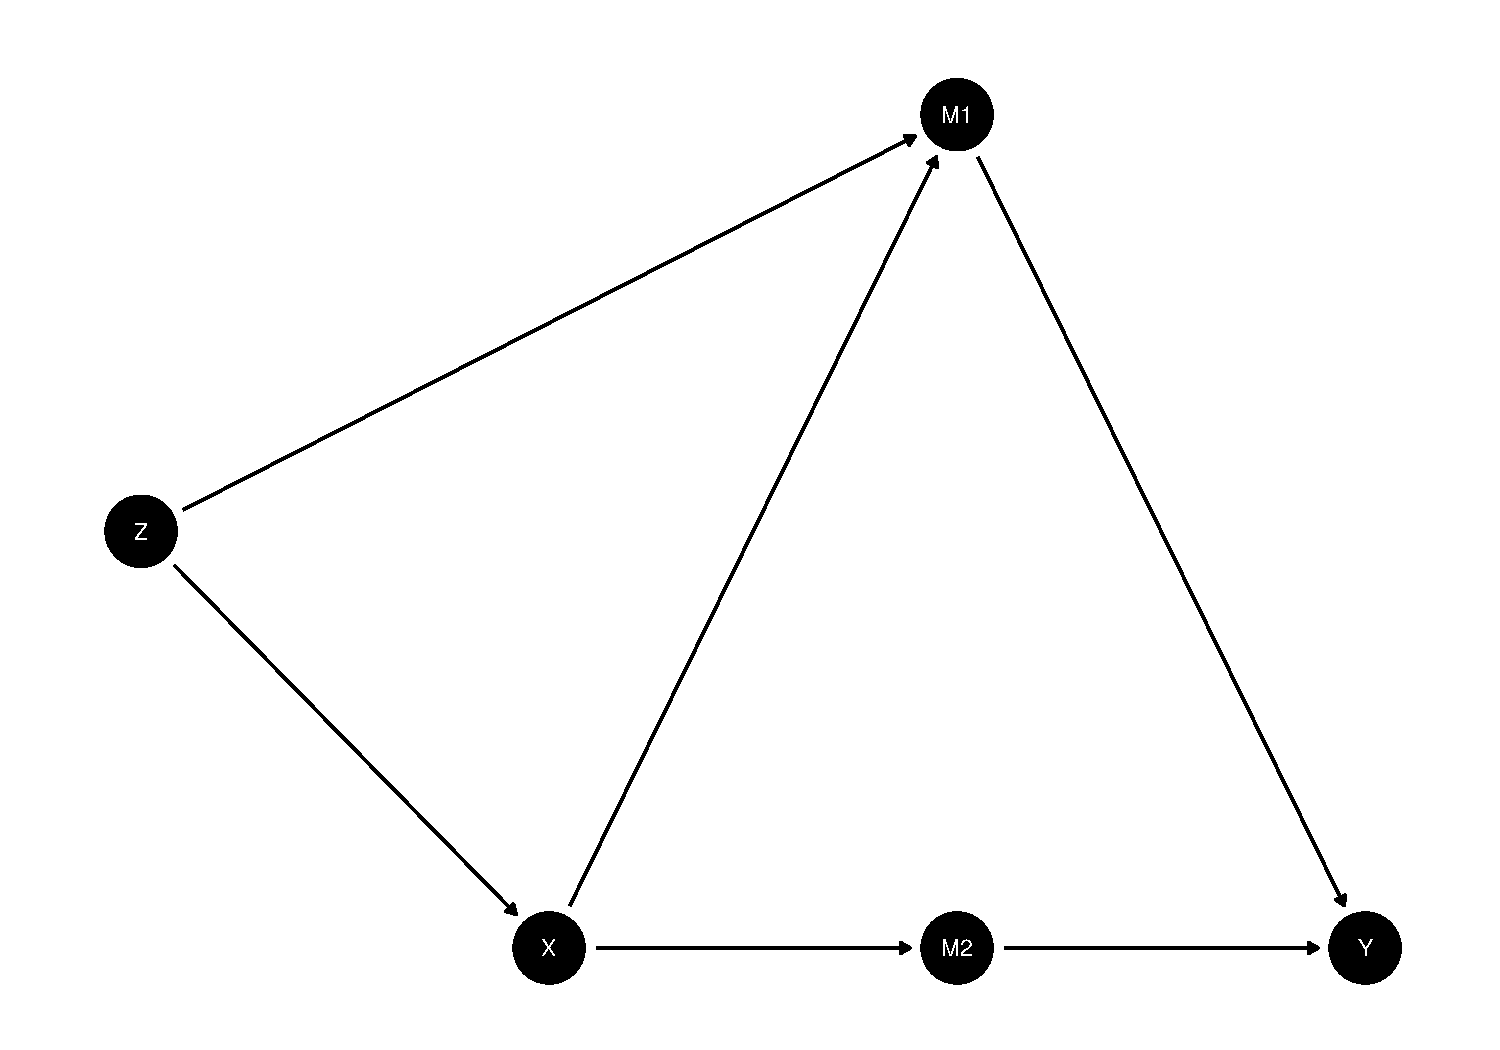
\includegraphics[width=0.7\textwidth,height=\textheight]{3.2_bayes_files/figure-beamer/unnamed-chunk-2-1.pdf}

}

\end{figure}

What's the probability of being a circle given you are black?
\end{frame}

\begin{frame}{Illustration 2. More formally.}
\protect\hypertarget{illustration-2.-more-formally.}{}
As an equation this might be written:

\[\text{Prob You have the Disease | Pos} = \frac{\text{How many have the disease and test pos?}}{\text{How many people test pos?}}\]
\end{frame}

\begin{frame}{Two Child Problem}
\protect\hypertarget{two-child-problem}{}
Consider last an old puzzle found described @gardner1961second.

\begin{itemize}
\tightlist
\item
  Mr Smith has two children, \(A\) and \(B\).
\item
  At least one of them is a boy.
\item
  What are the chances they are both boys?
\end{itemize}

To be explicit about the puzzle, we will assume that the information
that one child is a boy is given as a truthful answer to the question
``\emph{is at least one of the children a boy?}''

Assuming also that there is a 50\% probability that a given child is a
boy.
\end{frame}

\begin{frame}{Two Child Problem}
\protect\hypertarget{two-child-problem-1}{}
As an equation:

\[\text{Prob both boys | Not both girls} = \frac{\text{Prob both boys}}{\text{Prob not both girls}} = \frac{\text{1 in 4}}{\text{3 in 4}}\]
\end{frame}

\begin{frame}{Bayes Rule}
\protect\hypertarget{bayes-rule-1}{}
Formally, all of these equations are applications of Bayes' rule which
is a simple and powerful formula for deriving updated beliefs from new
data.

The formula is given as: \begin{eqnarray}
\Pr(H|\mathcal{D})&=&\frac{\Pr(\mathcal{D}|H)\Pr(H)}{\Pr(\mathcal{D})}\\
                  &=&\frac{\Pr(\mathcal{D}|H)\Pr(H)}{\sum_{H'}\Pr(\mathcal{D}|H')\Pr(H'))}
\end{eqnarray}
\end{frame}

\begin{frame}{Bayes Rule}
\protect\hypertarget{bayes-rule-2}{}
Formally, all of these equations are applications of Bayes' rule which
is a simple and powerful formula for deriving updated beliefs from new
data.

For continuous distributions and parameter vector \(\theta\):

\[p(\theta|\mathcal{D})=\frac{p(\mathcal{D}|\theta)p(\theta)}{\int_{\theta'}p(\mathcal{D|\theta'})p(\theta')d\theta}\]
\end{frame}

\begin{frame}{Useful Distributions: Beta and Dirichlet Distributions}
\protect\hypertarget{useful-distributions-beta-and-dirichlet-distributions}{}
\begin{itemize}
\tightlist
\item
  Bayes rule requires the ability to express a prior distribution but it
  does not require that the prior have any particular properties other
  than being probability distributions.
\item
  Sometimes however it can be useful to make use of ``off the shelf''
  distributions.
\end{itemize}

Consider \textbf{the share of people in a population that voted}. This
is a quantity between 0 and 1.

\begin{itemize}
\tightlist
\item
  Two people might may both believe that the turnout was around 50\% but
  differ in how certain they are about this claim.
\item
  One might claim to have no information and to believe any turnout rate
  between 0 and 100\% is equally likely; another might be completely
  confident that the number if 50\%.
\end{itemize}

Here the parameter of interest is a \emph{share}. The \textbf{Beta} and
\textbf{Dirichlet} distributions are particularly useful for
representing beliefs on shares.
\end{frame}

\begin{frame}{Beta}
\protect\hypertarget{beta}{}
\begin{itemize}
\tightlist
\item
  The Beta distribution is a distribution over the \([0,1]\) that is
  governed by two parameters, \(\alpha\) and \(\beta\).
\item
  In the case in which both \(\alpha\) and \(\beta\) are 1, the
  distribution is uniform -- all values are seen as equally likely.
\item
  As \(\alpha\) rises large outcomes are seen as more likely
\item
  As \(\beta\) rises, lower outcomes are seen as more likely.
\item
  If both rise proportionately the expected outcome does not change but
  the distribution becomes tighter.
\end{itemize}

An attractive feature is that if one has a prior Beta(\(\alpha\),
\(\beta\)) over the probability of some event, and then one observes a
positive case, the Bayesian posterior distribution is also a Beta with
with parameters \(\alpha+1, \beta\). Thus if people start with uniform
priors and build up knowledge on seeing outcomes, their posterior
beliefs should be Beta.
\end{frame}

\begin{frame}{Beta}
\protect\hypertarget{beta-1}{}
Figure \ref{betas} shows a set of such distributions.

\begin{figure}

{\centering 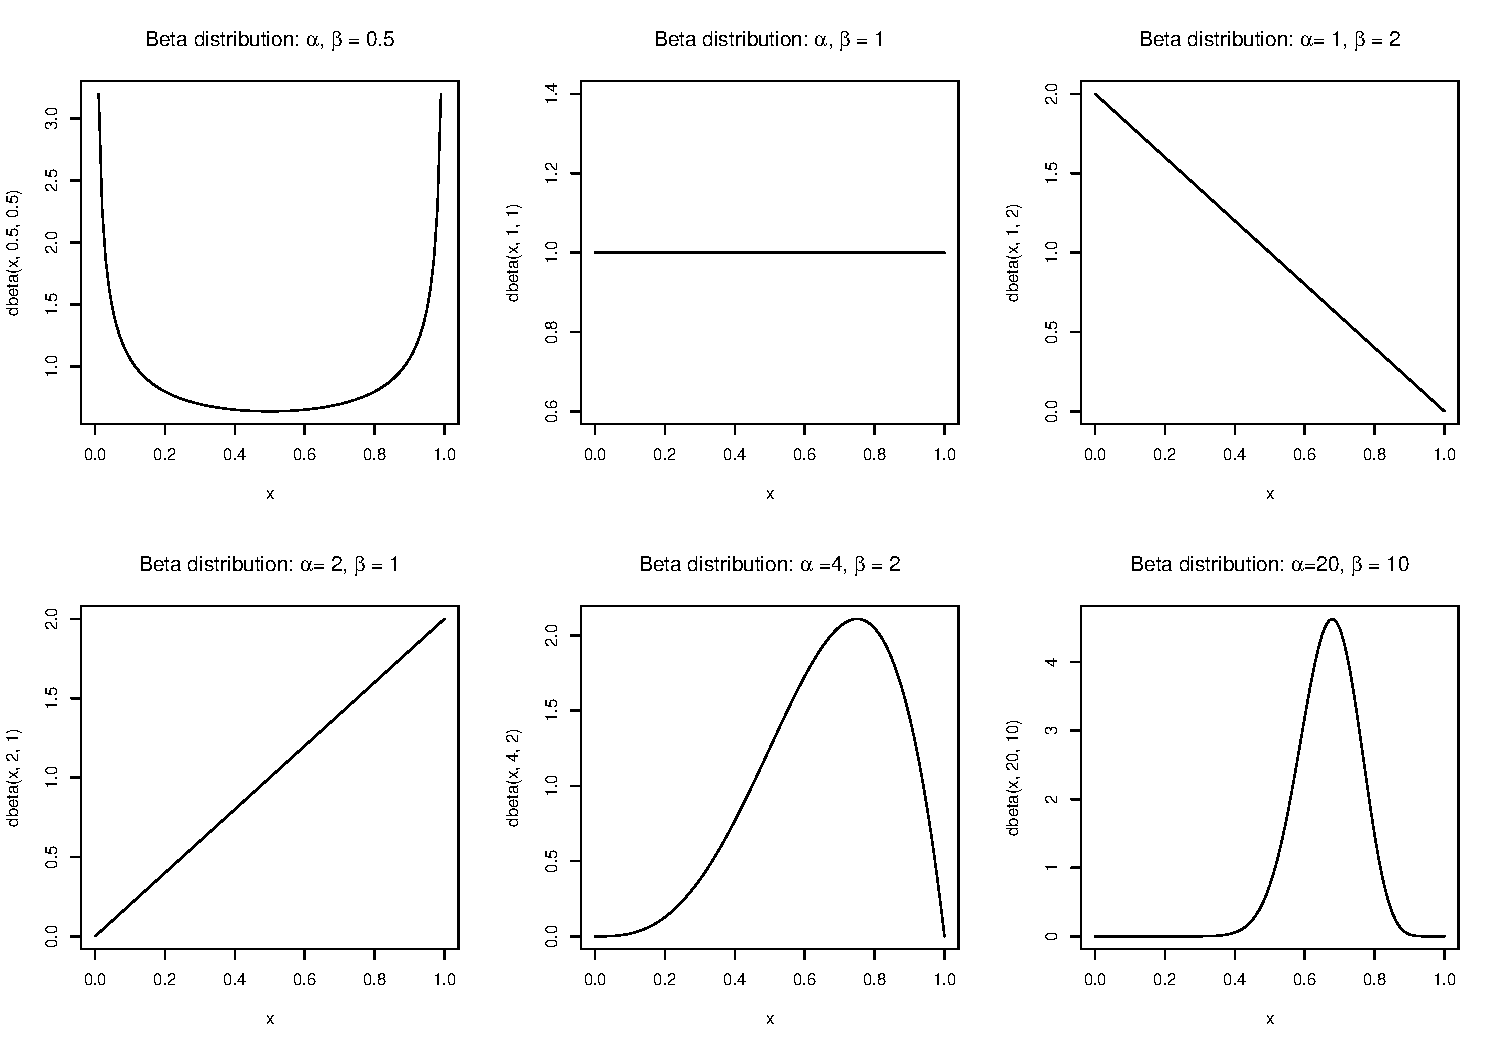
\includegraphics{3.2_bayes_files/figure-beamer/Betas-1.pdf}

}

\caption{\label{betas} Beta distributions}

\end{figure}
\end{frame}

\begin{frame}{Dirichlet distributions.}
\protect\hypertarget{dirichlet-distributions.}{}
The Dirichlet distributions are generalizations of the Beta to the
situation in which there are beliefs not just over a proportion, or a
probability, but over collections of probabilities.

\begin{itemize}
\item
  If four outcomes are possible and each is likely to occur with
  probability \(p_k\), \(k=1,2,3,4\) then beliefs are distributions over
  a three dimensional unit simplex.
\item
  The distribution has as many parameters as there are outcomes and
  these are traditionally recorded in a vector, \(\alpha\).
\item
  As with the Beta distribution, an uninformative prior (Jeffrey's
  prior) has \(\alpha\) parameters of \((.5,.5,.5, \dots)\) and a
  uniform (``flat'') distribution has \(\alpha = (1,1,1,,\dots)\).
\item
  The Dirichlet updates in a simple way. If you have a Dirichlet prior
  with parameter \(\alpha = (\alpha_1, \alpha_2, \dots)\) and you
  observe outcome \(1\), for example, then then posterior distribution
  is also Dirichlet with parameter vector
  \(\alpha' = (\alpha_1+1, \alpha_2,\dots)\).
\end{itemize}
\end{frame}

\hypertarget{a-bayes-exercises}{%
\subsection{3a Bayes Exercises}\label{a-bayes-exercises}}

\begin{frame}{PT by hand}
\protect\hypertarget{pt-by-hand}{}
\begin{enumerate}
\item
  \textbf{Simple process tracing}. Consider a ``hoop'' test: Say
  \(Pr(K|H) = 1, Pr(K|\neg H) = .5\). For each possible prior on
  \(p(H)\) over \(0,1\) graph your posterior or \(H\) if \(K\) is
  observed. Graph the posterior for when \(K\) is not observed.
\item
  \textbf{Simple correlation inference.} You know in a population that
  \(X=1\) about half the time and that \(Y=1\) about half the time;
  otherwise 0. Say you have a prior that puts equal weight on the
  possibilites that (a) \(X\) causes \(Y\) for all units (ie \(Y=1\) iff
  \(X=1\)), and (b) \(X\) and \(Y\) are orthogonal to each other.

  \begin{itemize}
  \tightlist
  \item
    What do you infer if you observe only one case and \(X \neq Y\)
  \item
    What do you infer if you observe only one case and \(X = Y\)
  \item
    What do you infer if you 100 cases and \(X = Y\) in 99 of these and
    \(X \neq Y\) in one of these? (Bonus: in this case what is the \(p\)
    value for the hypothesis that \(X\) does not cause \(Y\) )
  \end{itemize}
\end{enumerate}
\end{frame}

\hypertarget{stan}{%
\subsection{Stan}\label{stan}}

\begin{frame}{Plan}
\protect\hypertarget{plan}{}
In this short lecture we:

\begin{itemize}
\tightlist
\item
  fire up stan
\item
  implement a simple linear model and talk through the main model blocks
\item
  implement a simple hierarchical model
\item
  describe a behavioral game and set up a model to recover some
  parameters of interest, given the game
\end{itemize}
\end{frame}

\begin{frame}{Getting going}
\protect\hypertarget{getting-going}{}
\end{frame}

\begin{frame}[fragile]{Getting set up}
\protect\hypertarget{getting-set-up}{}
The good news: There is lots of help online. Start with:
https://github.com/stan-dev/rstan/wiki/RStan-Getting-Started

We will jump straight into things and work through a session.

\begin{enumerate}
\tightlist
\item
  Install the stan package and fire up. Useful to set options so that
  multiple cores are being used:
\end{enumerate}

\begin{Shaded}
\begin{Highlighting}[]
\FunctionTok{library}\NormalTok{(rstan)}
\FunctionTok{rstan\_options}\NormalTok{(}\AttributeTok{auto\_write =} \ConstantTok{TRUE}\NormalTok{)}
\FunctionTok{options}\NormalTok{(}\AttributeTok{mc.cores =}\NormalTok{ parallel}\SpecialCharTok{::}\FunctionTok{detectCores}\NormalTok{())}
\end{Highlighting}
\end{Shaded}
\end{frame}

\begin{frame}{One variable model: Simple example}
\protect\hypertarget{one-variable-model-simple-example}{}
\begin{enumerate}
\setcounter{enumi}{1}
\tightlist
\item
  Now lets consider the simplest one var linear model.

  \begin{itemize}
  \tightlist
  \item
    We will need model code
  \item
    And data
  \end{itemize}
\end{enumerate}
\end{frame}

\begin{frame}{A simple model: Code}
\protect\hypertarget{a-simple-model-code}{}
To implement a stan model you should write the code in a text editor and
save it as a text file. You can also write it directly in your script.
You can then bring the file into R or call the file directly.

\begin{itemize}
\tightlist
\item
  There are many examples of stan models here:

  \begin{itemize}
  \tightlist
  \item
    https://github.com/stan-dev/example-models/tree/master/ARM/Ch.4
  \item
    https://github.com/stan-dev/example-models/wiki
  \end{itemize}
\end{itemize}
\end{frame}

\begin{frame}[fragile]{A simple model: Code}
\protect\hypertarget{a-simple-model-code-1}{}
I saved a simple model called \texttt{one\_var.stan} locally. Here it
is:

\begin{Shaded}
\begin{Highlighting}[]
\FunctionTok{readLines}\NormalTok{(}\StringTok{"assets/one\_var.stan"}\NormalTok{, }\AttributeTok{warn =} \ConstantTok{FALSE}\NormalTok{) }\SpecialCharTok{|\textgreater{}}
    \FunctionTok{cat}\NormalTok{(}\AttributeTok{sep =} \StringTok{"}\SpecialCharTok{\textbackslash{}n}\StringTok{"}\NormalTok{)}
\end{Highlighting}
\end{Shaded}

data \{ int\textless lower=0\textgreater{} N; vector{[}N{]} Y;
vector{[}N{]} X; \} parameters \{ real a; real b;
real\textless lower=0\textgreater{} sigma; \} model \{ Y
\textasciitilde{} normal(a + b * X, sigma); \}
\end{frame}

\begin{frame}[fragile]{A simple model: Code}
\protect\hypertarget{a-simple-model-code-2}{}
The key features here are (read from bottom up!):

\begin{itemize}
\tightlist
\item
  \(Y\) is assumed to be normally distributed with mean
  \texttt{a\ +\ bX} and standard deviation \texttt{sigma}.
\item
  There are then three parameters: \texttt{a}, \texttt{b},
  \texttt{sigma}.
\item
  There are no priors placed on these but sigma is constrained to be
  positive. Without priors improper flat priors are assumed.
\item
  Stan expects a data set that contains three things: a scalar,
  \texttt{N} and \texttt{X1,}Y` data
\end{itemize}
\end{frame}

\begin{frame}[fragile]{Simple model: Data}
\protect\hypertarget{simple-model-data}{}
We feed data to the model in the form of a list. The idea of a list is
that the data can include all sorts of objects, not just a single
dataset.

\begin{Shaded}
\begin{Highlighting}[]
\NormalTok{X }\OtherTok{=} \FunctionTok{rnorm}\NormalTok{(}\DecValTok{20}\NormalTok{)}

\NormalTok{some\_data }\OtherTok{\textless{}{-}} \FunctionTok{list}\NormalTok{(}\AttributeTok{N =} \DecValTok{20}\NormalTok{, }\AttributeTok{X =}\NormalTok{ X, }\AttributeTok{Y =}\NormalTok{ X }\SpecialCharTok{+} \FunctionTok{rnorm}\NormalTok{(}\DecValTok{20}\NormalTok{))}
\end{Highlighting}
\end{Shaded}
\end{frame}

\begin{frame}[fragile]{Simple model: Now let's Run It}
\protect\hypertarget{simple-model-now-lets-run-it}{}
\begin{Shaded}
\begin{Highlighting}[]
\NormalTok{M }\OtherTok{\textless{}{-}} \FunctionTok{stan}\NormalTok{(}\AttributeTok{file =} \StringTok{"assets/one\_var.stan"}\NormalTok{, }\AttributeTok{data =}\NormalTok{ some\_data)}
\end{Highlighting}
\end{Shaded}

When you run the model you get a lot of useful output on the estimation
and the posterior distribution. Here though are the key results:

\begin{tabular}{l|r|r|r}
\hline
  & mean & sd & Rhat\\
\hline
a & -0.179 & 0.214 & 1\\
\hline
b & 0.738 & 0.183 & 1\\
\hline
sigma & 0.950 & 0.175 & 1\\
\hline
\end{tabular}

These look good.

The Rhat at the end tells you about convergence. You want this very
close to 1.
\end{frame}

\begin{frame}[fragile]{A simple model: Now lets use it}
\protect\hypertarget{a-simple-model-now-lets-use-it}{}
The model output contains the full posterior distribution.

\begin{Shaded}
\begin{Highlighting}[]
\NormalTok{my\_posterior }\OtherTok{\textless{}{-}}\NormalTok{ M }\SpecialCharTok{|\textgreater{}}
    \FunctionTok{extract}\NormalTok{() }\SpecialCharTok{|\textgreater{}}
    \FunctionTok{data.frame}\NormalTok{()}

\NormalTok{my\_posterior }\SpecialCharTok{|\textgreater{}}
    \FunctionTok{ggplot}\NormalTok{(}\FunctionTok{aes}\NormalTok{(a, b)) }\SpecialCharTok{+} \FunctionTok{geom\_point}\NormalTok{()}
\end{Highlighting}
\end{Shaded}

\begin{figure}

{\centering 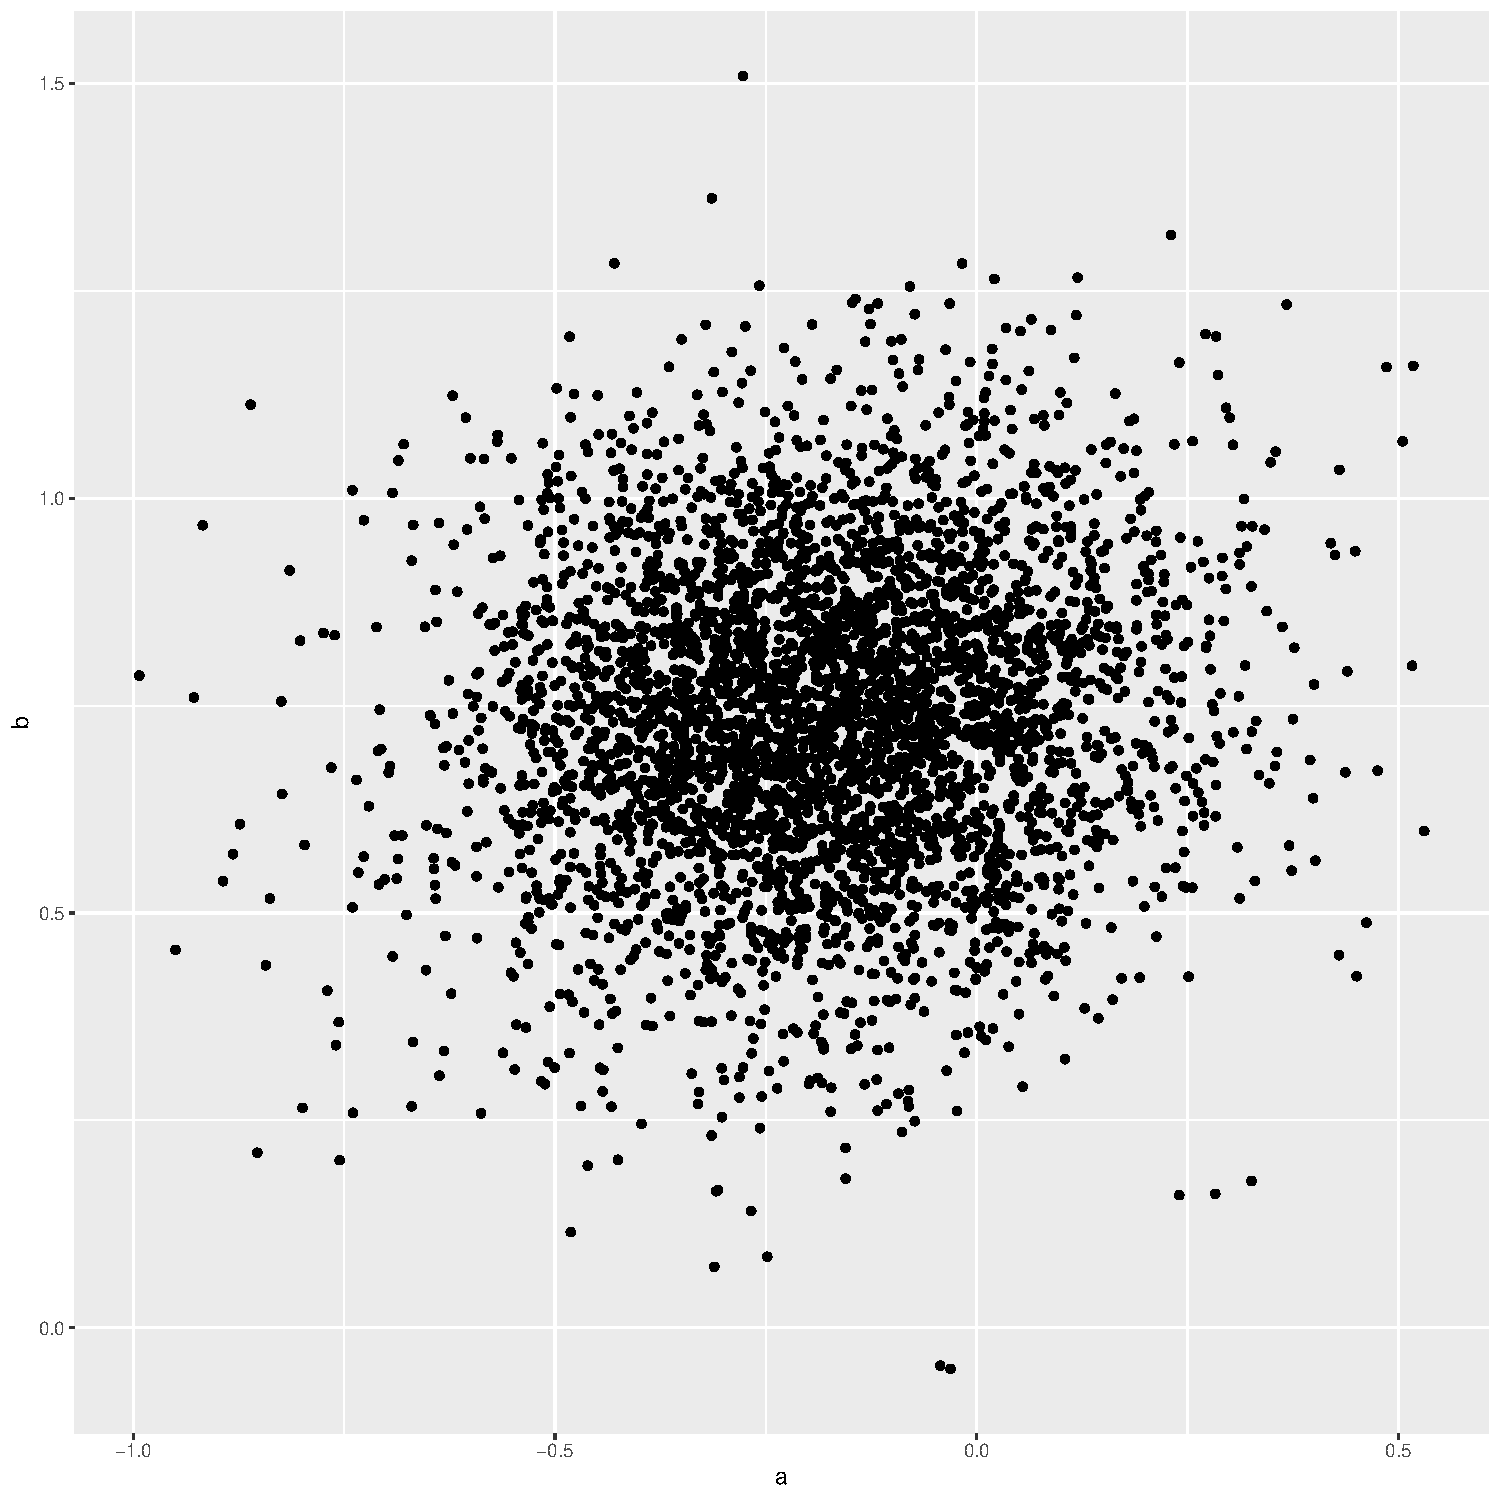
\includegraphics[width=0.5\textwidth,height=\textheight]{3.2_bayes_files/figure-beamer/figposta-1.pdf}

}

\end{figure}
\end{frame}

\begin{frame}[fragile]{A simple model: Now lets use it}
\protect\hypertarget{a-simple-model-now-lets-use-it-1}{}
With the full posterior you can can look at marginal posterior
distributions over arbitrary transformations of parameters.

\begin{Shaded}
\begin{Highlighting}[]
\FunctionTok{summary}\NormalTok{((my\_posterior}\SpecialCharTok{$}\NormalTok{a }\SpecialCharTok{+}\NormalTok{ my\_posterior}\SpecialCharTok{$}\NormalTok{b)}\SpecialCharTok{/}\NormalTok{my\_posterior}\SpecialCharTok{$}\NormalTok{a)}
\end{Highlighting}
\end{Shaded}

\begin{verbatim}
 Min.   1st Qu.    Median      Mean   3rd Qu.      Max. 
\end{verbatim}

-2528.863 -3.834 -1.454 0.429 -0.159 6552.412
\end{frame}

\begin{frame}[fragile]{Building up}
\protect\hypertarget{building-up}{}
Let's go back to the code.

There we had three key blocks: \texttt{data}, \texttt{parameters}, and
\texttt{model}

More generally the blocks you can specify are:

\begin{itemize}
\tightlist
\item
  \texttt{data} (define the vars that will be coming in from the data
  list)
\item
  \texttt{transformed\ data} (can be used for preprocessing)
\item
  \texttt{parameters} (required: defines the parameters to be estimated)
\item
  \texttt{transformed\ parameters} (transformations of parameters useful
  for computational reasons and sometimes for clarity)
\item
  \texttt{model} (give priors and likelihood)
\item
  \texttt{generated\ quantities} (can be used for post processing)
\end{itemize}
\end{frame}

\begin{frame}[fragile]{Parameters block}
\protect\hypertarget{parameters-block}{}
The parameters block declared the set of parameters that we wanted to
estimate. In the simple model these were \texttt{a}, \texttt{b}, and
\texttt{sigma}. Note in the declaration we also:

\begin{itemize}
\tightlist
\item
  said what kind of parameters they (vectors, matrices, simplices etc)
\item
  gave possible constraints
\end{itemize}
\end{frame}

\begin{frame}[fragile]{Parameters block}
\protect\hypertarget{parameters-block-1}{}
Instead of defining:

\begin{Shaded}
\begin{Highlighting}[]
\NormalTok{real a;}
\NormalTok{real b;}
\end{Highlighting}
\end{Shaded}

We could have defined

\begin{Shaded}
\begin{Highlighting}[]
\NormalTok{vector[}\DecValTok{2}\NormalTok{] coefs;}
\end{Highlighting}
\end{Shaded}

and then referenced \texttt{coef{[}1{]}} and \texttt{coef{[}2{]}} in the
model block.
\end{frame}

\begin{frame}[fragile]{Parameters block}
\protect\hypertarget{parameters-block-2}{}
Or we could also have imposed the constraint that the slope coefficient
is positive by defining:

\begin{Shaded}
\begin{Highlighting}[]
\NormalTok{real a;}
\NormalTok{real}\SpecialCharTok{\textless{}}\NormalTok{lower }\OtherTok{=} \DecValTok{0}\SpecialCharTok{\textgreater{}}\NormalTok{ b;}
\end{Highlighting}
\end{Shaded}
\end{frame}

\begin{frame}[fragile]{Model Block}
\protect\hypertarget{model-block}{}
In the model block we give the likelihood

But we can also give the priors (if we want to). If priors are not
provided, flat (possibly improper) priors are assumed

In our case for example we could have provided something like

\begin{Shaded}
\begin{Highlighting}[]
\NormalTok{model \{}
\NormalTok{  b }\SpecialCharTok{\textasciitilde{}} \FunctionTok{normal}\NormalTok{(}\SpecialCharTok{{-}}\DecValTok{10}\NormalTok{, }\DecValTok{1}\NormalTok{);}
\NormalTok{  Y }\SpecialCharTok{\textasciitilde{}} \FunctionTok{normal}\NormalTok{(a }\SpecialCharTok{+}\NormalTok{ b }\SpecialCharTok{*}\NormalTok{ X, sigma);}
\NormalTok{\}}
\end{Highlighting}
\end{Shaded}

This suggests that we start off believing \texttt{b} is centered on -10.
That will surely matter for our conclusions. Lets try it:
\end{frame}

\begin{frame}[fragile]{Version 2}
\protect\hypertarget{version-2}{}
This time I will write the model right in the editor:

\begin{Shaded}
\begin{Highlighting}[]
\NormalTok{new\_model }\OtherTok{\textless{}{-}} \StringTok{"}
\StringTok{data \{}
\StringTok{  int\textless{}lower=0\textgreater{} N;}
\StringTok{  vector[N] Y;}
\StringTok{  vector[N] X;}
\StringTok{\}}
\StringTok{parameters \{}
\StringTok{  real a;}
\StringTok{  real b;}
\StringTok{  real\textless{}lower=0\textgreater{} sigma;}
\StringTok{\}}
\StringTok{model \{}
\StringTok{  b \textasciitilde{} normal({-}10,1);}
\StringTok{  Y \textasciitilde{} normal(a + b * X, sigma);}
\StringTok{\}}
\StringTok{"}
\end{Highlighting}
\end{Shaded}
\end{frame}

\begin{frame}[fragile]{Estimation 2}
\protect\hypertarget{estimation-2}{}
\begin{Shaded}
\begin{Highlighting}[]
\NormalTok{M2 }\OtherTok{\textless{}{-}} \FunctionTok{stan}\NormalTok{(}\AttributeTok{model\_code =}\NormalTok{ new\_model, }\AttributeTok{data =}\NormalTok{ some\_data)}
\end{Highlighting}
\end{Shaded}

\begin{tabular}{l|r|r|r}
\hline
  & mean & sd & Rhat\\
\hline
a & -1.338 & 2.444 & 1.003\\
\hline
b & -7.875 & 1.172 & 1.003\\
\hline
sigma & 10.988 & 2.499 & 1.001\\
\hline
\end{tabular}

Note that we get a much lower estimate for \texttt{b} with the same
data.
\end{frame}

\begin{frame}{A multilevel model}
\protect\hypertarget{a-multilevel-model}{}
Now imagine a setting in which there are 10 villages, each with 10
respondents. Half in each village are assigned to treatment \(X=1\), and
half to control \(X=0\).

Say that there is possible a village specific average outcome:
\(Y_v = a_v + b_vX\) where \(a_v\) and \(b_v\) are each draw from some
distribution with a mean and variance of interest. The individual
outcomes are draws from a village level distribution centered on the
village specific average outcome.

This all implies a multilevel structure.
\end{frame}

\begin{frame}[fragile]{A ml model}
\protect\hypertarget{a-ml-model}{}
Here is a model for this

\tiny

\begin{Shaded}
\begin{Highlighting}[]
\NormalTok{ml\_model }\OtherTok{\textless{}{-}} \StringTok{"}
\StringTok{data \{}
\StringTok{  vector[100] Y;}
\StringTok{  int\textless{}lower=0,upper=1\textgreater{} X[100];}
\StringTok{  int village[100];}
\StringTok{\}}
\StringTok{parameters \{}
\StringTok{  vector\textless{}lower=0\textgreater{}[3] sigma; }
\StringTok{  vector[10] a;}
\StringTok{  vector[10] b;}
\StringTok{  real mu\_a;}
\StringTok{  real mu\_b;}
\StringTok{\}}
\StringTok{transformed parameters \{}
\StringTok{  vector[100] Y\_vx;}
\StringTok{  for (i in 1:100) Y\_vx[i] = a[village[i]] + b[village[i]] * X[i];}
\StringTok{\}}
\StringTok{model \{}
\StringTok{  a \textasciitilde{} normal(mu\_a, sigma[1]);}
\StringTok{  b \textasciitilde{} normal(mu\_b, sigma[2]);}
\StringTok{  Y \textasciitilde{} normal(Y\_vx, sigma[3]);}
\StringTok{\}}
\StringTok{"}
\end{Highlighting}
\end{Shaded}

Here is a slightly more general version:
https://github.com/stan-dev/example-models/blob/master/ARM/Ch.17/17.1\_radon\_vary\_inter\_slope.stan
\end{frame}

\begin{frame}[fragile]{Multilevel model: Data}
\protect\hypertarget{multilevel-model-data}{}
Lets create some multilevel data. Looking at this, can you tell what is
the typical village level effect? How much heterogeneity is there?

\begin{Shaded}
\begin{Highlighting}[]
\NormalTok{village }\OtherTok{\textless{}{-}} \FunctionTok{rep}\NormalTok{(}\DecValTok{1}\SpecialCharTok{:}\DecValTok{10}\NormalTok{, }\AttributeTok{each =} \DecValTok{10}\NormalTok{)}
\NormalTok{village\_b }\OtherTok{\textless{}{-}} \DecValTok{1} \SpecialCharTok{+} \FunctionTok{rnorm}\NormalTok{(}\DecValTok{10}\NormalTok{)}
\NormalTok{X }\OtherTok{\textless{}{-}} \FunctionTok{rep}\NormalTok{(}\DecValTok{0}\SpecialCharTok{:}\DecValTok{1}\NormalTok{, }\DecValTok{50}\NormalTok{)}
\NormalTok{Y }\OtherTok{\textless{}{-}}\NormalTok{ village\_b[village] }\SpecialCharTok{*}\NormalTok{ X }\SpecialCharTok{+} \FunctionTok{rnorm}\NormalTok{(}\DecValTok{100}\NormalTok{)}

\NormalTok{ml\_data }\OtherTok{\textless{}{-}} \FunctionTok{list}\NormalTok{(}\AttributeTok{village =}\NormalTok{ village, }\AttributeTok{X =}\NormalTok{ X, }\AttributeTok{Y =}\NormalTok{ Y)}
\end{Highlighting}
\end{Shaded}
\end{frame}

\begin{frame}[fragile]{Multilevel Results}
\protect\hypertarget{multilevel-results}{}
\begin{Shaded}
\begin{Highlighting}[]
\NormalTok{M\_ml }\OtherTok{\textless{}{-}} \FunctionTok{stan}\NormalTok{(}\AttributeTok{model\_code =}\NormalTok{ ml\_model, }\AttributeTok{data =}\NormalTok{ ml\_data)}
\end{Highlighting}
\end{Shaded}

\begin{tabular}{l|r|r|r}
\hline
  & mean & sd & Rhat\\
\hline
mu\_a & -0.29 & 0.25 & 1.00\\
\hline
mu\_b & 1.89 & 0.26 & 1.00\\
\hline
sigma[1] & 0.61 & 0.25 & 1.00\\
\hline
sigma[2] & 0.47 & 0.28 & 1.01\\
\hline
sigma[3] & 0.98 & 0.08 & 1.00\\
\hline
\end{tabular}
\end{frame}

\begin{frame}{A game and a structural model}
\protect\hypertarget{a-game-and-a-structural-model}{}
Say that a set of people in a population are playing sequential
prisoner's dilemmas.

In such games selfish behavior might suggest defections by everyone
everywhere. But of course people often cooperate. Why might this be?

\begin{itemize}
\tightlist
\item
  One possible reason is that some people are irrational, in the sense
  that they simply choose to cooperate, ignoring the payoffs.
\item
  Another possibility is that rational people think that others are
  irrational, in the sense that they think that others will reciprocate
  when they observe cooperative action
\end{itemize}
\end{frame}

\begin{frame}{Model}
\protect\hypertarget{model}{}
We will capture some of this intuition with a behavioral type model in
which

\begin{itemize}
\tightlist
\item
  each player has a ``rationality'' propensity of \(r_i\) -- this is the
  probability with which they choose to do the rational thing, rather
  than the generous thing
\item
  \(r_i \sim U[0, \theta]\) for \(\theta > .5\).
\item
  A player with rationality propensity of \(r_i\) believes
  \(r_j \sim [0, r_i]\). So everyone assumes that they are the most
  rational people in the room\ldots{}
\item
  The game is such that: * second mover: a second mover with rationality
  propensity \(r_i\) will cooperate with probability \(1-r_i\) if the
  first mover cooperated; otherwise they defect * first mover: a first
  mover with \(r_i\) will cooperate nonstrategically with probability
  \((1-r_i)\); however with probability \(r_i\) they will also cooperate
  \emph{strategically} if they think that the second mover has
  \(r_j<.25\).
\end{itemize}
\end{frame}

\begin{frame}{Expectations from model}
\protect\hypertarget{expectations-from-model}{}
In all, this means that a player with propensity \(r_i>.5\) will
cooperate with probability \(1-r_i\); a player with propensity
\(r_i<.5\) will cooperate with probability \(1\).

Interestingly the not-very-rational people sometimes cooperate
strategically but the really rational people never cooperate
strategically because they think it won't work.
\end{frame}

\begin{frame}{Event Probabilities}
\protect\hypertarget{event-probabilities}{}
What then are the probabilities of each of the possible outcomes?

\begin{itemize}
\tightlist
\item
  There will be cooperation by \emph{both} players with probability
  \((\int_0^{.5} p(r_i) dr_i + \int_{.5}^1 p(r_i)(1-r_i) dr_i)\int_0^1p(r_i)(1-r_i)dr_i\)
\item
  There will be cooperation by player 1 only with probability
  \((\int_0^{.5} p(r_i) dr_i + \int_{.5}^1 p(r_i)(1-r_i) dr_i)(\int_0^1p(r_i)(r_i)dr_i)\)
\item
  There will be cooperation by neither with probability:
  \(1-\int_0^{.5} p(r_i) dr_i - \int_{.5}^1 p(r_i)(1-r_i) dr_i\)
\end{itemize}

where \(p\) is the density function on \(r_i\) given \(\theta\)
\end{frame}

\begin{frame}{Event probabilities}
\protect\hypertarget{event-probabilities-1}{}
Given the assumption on \(p\)

\begin{itemize}
\tightlist
\item
  There will be cooperation by \emph{both} players with probability
  \((1+.25/\theta -.5\theta)(1-.5\theta)\)
\item
  There will be cooperation by player 1 only with probability
  \((1+.25/\theta -.5\theta)(.5\theta)\)
\item
  There will be cooperation by neither player with probability
  \((.5\theta-.25/\theta)\)
\end{itemize}
\end{frame}

\begin{frame}{Data}
\protect\hypertarget{data}{}
\begin{itemize}
\item
  We have data on the actions of the first movers and the second movers
  and are interested in the distribution of the \(p_i\)s.
\item
  Lets collapse that data into a simple list of the number of each type
  of game outcome:
\item
  And say we start off with a uniform prior of \(\theta\).
\item
  What should we conclude about \(\theta\)?
\end{itemize}
\end{frame}

\begin{frame}[fragile]{Model}
\protect\hypertarget{model-1}{}
Here's a model:

\tiny

\begin{Shaded}
\begin{Highlighting}[]
\NormalTok{game\_model }\OtherTok{\textless{}{-}} \StringTok{"}
\StringTok{data \{}
\StringTok{  int\textless{}lower=0\textgreater{} play[3];}
\StringTok{\}}
\StringTok{parameters \{}
\StringTok{  real\textless{}lower=.5, upper=1\textgreater{} theta;}
\StringTok{\}}
\StringTok{transformed parameters \{}
\StringTok{simplex[3] w;}
\StringTok{ w[1] = (1+.25*theta {-} .5*theta)*(1{-}.5*theta);}
\StringTok{ w[2] = (1+.25*theta {-} .5*theta)*(.5*theta);}
\StringTok{ w[3] = ({-}.25*theta  + .5*theta);}
\StringTok{\}}
\StringTok{model \{}
\StringTok{  play \textasciitilde{} multinomial(w);}
\StringTok{\}}
\StringTok{"}
\end{Highlighting}
\end{Shaded}

Note we define event weights as transformed parameters on a simplex. We
also constrain \(\theta\) to be \(>.5\). Obviously we are relying
\emph{a lot} on our model.
\end{frame}

\begin{frame}[fragile]{Plot posterior on \(\theta\)}
\protect\hypertarget{plot-posterior-on-theta}{}
\begin{Shaded}
\begin{Highlighting}[]
\NormalTok{M3 }\OtherTok{\textless{}{-}} \FunctionTok{stan}\NormalTok{(}\AttributeTok{model\_code =}\NormalTok{ game\_model, }\AttributeTok{data =} \FunctionTok{list}\NormalTok{(}\AttributeTok{play =} \FunctionTok{c}\NormalTok{(}\DecValTok{10}\NormalTok{,}
    \DecValTok{10}\NormalTok{, }\DecValTok{10}\NormalTok{)))}
\end{Highlighting}
\end{Shaded}

\begin{figure}

{\centering \includegraphics[width=0.5\textwidth,height=\textheight]{3.2_bayes_files/figure-beamer/unnamed-chunk-27-1.pdf}

}

\end{figure}
\end{frame}

\begin{frame}[fragile]{Plot posterior on \(\theta\)}
\protect\hypertarget{plot-posterior-on-theta-1}{}
\begin{Shaded}
\begin{Highlighting}[]
\NormalTok{M4 }\OtherTok{\textless{}{-}} \FunctionTok{stan}\NormalTok{(}\AttributeTok{model\_code =}\NormalTok{ game\_model, }\AttributeTok{data =} \FunctionTok{list}\NormalTok{(}\AttributeTok{play =} \FunctionTok{c}\NormalTok{(}\DecValTok{20}\NormalTok{,}
    \DecValTok{6}\NormalTok{, }\DecValTok{4}\NormalTok{)))}
\end{Highlighting}
\end{Shaded}

\begin{figure}

{\centering \includegraphics[width=0.5\textwidth,height=\textheight]{3.2_bayes_files/figure-beamer/unnamed-chunk-29-1.pdf}

}

\end{figure}
\end{frame}

\begin{frame}{Posterior on a quantity of interest}
\protect\hypertarget{posterior-on-a-quantity-of-interest}{}
What is the probability of observing \emph{strategic} first round
cooperation?

A player with rationality \(r_i\) will cooperate strategically with
probability \(r_i\) if \(r_i<.5\) and 0 otherwise. Thus we are
interested in \(\int_0^{.5}r_i/\theta dr_i = .125/\theta\)

\begin{figure}

{\centering \includegraphics[width=0.5\textwidth,height=\textheight]{3.2_bayes_files/figure-beamer/unnamed-chunk-30-1.pdf}

}

\end{figure}
\end{frame}

\hypertarget{stan-1}{%
\subsection{Stan}\label{stan-1}}

\begin{frame}[fragile]{Getting set up}
\protect\hypertarget{getting-set-up-1}{}
The good news: There is lots of help online. Start with:
https://github.com/stan-dev/rstan/wiki/RStan-Getting-Started

We will jump straight into things and work through a session.

\begin{enumerate}
\tightlist
\item
  Install the stan package and fire up. Useful to set options so that
  multiple cores are being used:
\end{enumerate}

\begin{Shaded}
\begin{Highlighting}[]
\FunctionTok{library}\NormalTok{(rstan)}
\FunctionTok{rstan\_options}\NormalTok{(}\AttributeTok{auto\_write =} \ConstantTok{TRUE}\NormalTok{)}
\FunctionTok{options}\NormalTok{(}\AttributeTok{mc.cores =}\NormalTok{ parallel}\SpecialCharTok{::}\FunctionTok{detectCores}\NormalTok{())}
\end{Highlighting}
\end{Shaded}
\end{frame}

\begin{frame}{One variable model: Simple example}
\protect\hypertarget{one-variable-model-simple-example-1}{}
\begin{enumerate}
\setcounter{enumi}{1}
\tightlist
\item
  Now lets consider the simplest one var linear model.

  \begin{itemize}
  \tightlist
  \item
    We will need model code
  \item
    And data
  \end{itemize}
\end{enumerate}
\end{frame}

\begin{frame}{A simple model: Code}
\protect\hypertarget{a-simple-model-code-3}{}
To implement a stan model you should write the code in a text editor and
save it as a text file. You can also write it directly in your script.
You can then bring the file into R or call the file directly.

\begin{itemize}
\tightlist
\item
  There are many examples of stan models here:

  \begin{itemize}
  \tightlist
  \item
    https://github.com/stan-dev/example-models/tree/master/ARM/Ch.4
  \item
    https://github.com/stan-dev/example-models/wiki
  \end{itemize}
\end{itemize}
\end{frame}

\begin{frame}[fragile]{A simple model: Code}
\protect\hypertarget{a-simple-model-code-4}{}
I saved a simple model called \texttt{one\_var.stan} locally. Here it
is:

\begin{Shaded}
\begin{Highlighting}[]
\FunctionTok{print}\NormalTok{(}\FunctionTok{stan\_model}\NormalTok{(}\AttributeTok{file =} \StringTok{"stan\_models/one\_var.stan"}\NormalTok{))}
\end{Highlighting}
\end{Shaded}

Error in file(fname, ``rt'') : cannot open the connection

\begin{verbatim}
Error in get_model_strcode(file, model_code): cannot open model file "C:\Dropbox\Teaching\Humboldt\2024_advanced_ci\slides\stan_models\one_var.stan"
\end{verbatim}
\end{frame}

\begin{frame}[fragile]{A simple model: Code}
\protect\hypertarget{a-simple-model-code-5}{}
The key features here are (read from bottom up!):

\begin{itemize}
\tightlist
\item
  \(Y\) is assumed to be normally distributed with mean \texttt{a+bX}
  and standard deviation \texttt{sigma}.
\item
  There are then three parameters: \texttt{a}, \texttt{b},
  \texttt{sigma}.
\item
  There are no priors placed on these but sigma is constrained to be
  positive. Without priors improper flat priors are assumed.
\item
  Stan expects a data set that contains three things: a scalar,
  \texttt{N} and \texttt{X1,}Y` data
\end{itemize}
\end{frame}

\begin{frame}[fragile]{Simple model: Data}
\protect\hypertarget{simple-model-data-1}{}
We feed data to the model in the form of a list. The idea of a list is
that the data can include all sorts of objects, not just a single
dataset.

\begin{Shaded}
\begin{Highlighting}[]
\NormalTok{X }\OtherTok{=} \FunctionTok{rnorm}\NormalTok{(}\DecValTok{20}\NormalTok{)}

\NormalTok{some\_data }\OtherTok{\textless{}{-}} \FunctionTok{list}\NormalTok{(}\AttributeTok{N =} \DecValTok{20}\NormalTok{, }\AttributeTok{X =}\NormalTok{ X, }\AttributeTok{Y =}\NormalTok{ X }\SpecialCharTok{+} \FunctionTok{rnorm}\NormalTok{(}\DecValTok{20}\NormalTok{))}
\end{Highlighting}
\end{Shaded}
\end{frame}

\begin{frame}[fragile]{Simple model: Now let's Run It}
\protect\hypertarget{simple-model-now-lets-run-it-1}{}
\begin{Shaded}
\begin{Highlighting}[]
\NormalTok{M }\OtherTok{\textless{}{-}} \FunctionTok{stan}\NormalTok{(}\AttributeTok{file =} \StringTok{"stan\_models/one\_var.stan"}\NormalTok{, }\AttributeTok{data =}\NormalTok{ some\_data)}
\end{Highlighting}
\end{Shaded}

Error in file(fname, ``rt'') : cannot open the connection

\begin{verbatim}
Error in get_model_strcode(file, model_code): cannot open model file "C:\Dropbox\Teaching\Humboldt\2024_advanced_ci\slides\stan_models\one_var.stan"
\end{verbatim}

When you run the model you get a lot of useful output on the estimation
and the posterior distribution. Here though are the key results:

\begin{tabular}{l|r|r|r}
\hline
  & mean & sd & Rhat\\
\hline
a & -0.179 & 0.214 & 1\\
\hline
b & 0.738 & 0.183 & 1\\
\hline
sigma & 0.950 & 0.175 & 1\\
\hline
\end{tabular}

These look good.

The Rhat at the end tells you about convergence. You want this very
close to 1.
\end{frame}

\begin{frame}[fragile]{A simple model: Now lets use it}
\protect\hypertarget{a-simple-model-now-lets-use-it-2}{}
The model output contains the full posterior distribution.

\begin{Shaded}
\begin{Highlighting}[]
\NormalTok{my\_posterior }\OtherTok{\textless{}{-}} \FunctionTok{extract}\NormalTok{(M)}
\FunctionTok{plot}\NormalTok{(my\_posterior}\SpecialCharTok{$}\NormalTok{a, my\_posterior}\SpecialCharTok{$}\NormalTok{b)}
\end{Highlighting}
\end{Shaded}

\begin{figure}

{\centering \includegraphics[width=0.5\textwidth,height=\textheight]{3.2_bayes_files/figure-beamer/figpostb-1.pdf}

}

\end{figure}
\end{frame}

\begin{frame}[fragile]{A simple model: Now lets use it}
\protect\hypertarget{a-simple-model-now-lets-use-it-3}{}
With the full posterior you can can look at marginal posterior
distributions over arbitrary transformations of parameters.

\begin{Shaded}
\begin{Highlighting}[]
\FunctionTok{summary}\NormalTok{((my\_posterior}\SpecialCharTok{$}\NormalTok{a }\SpecialCharTok{+}\NormalTok{ my\_posterior}\SpecialCharTok{$}\NormalTok{b)}\SpecialCharTok{/}\NormalTok{my\_posterior}\SpecialCharTok{$}\NormalTok{a)}
\end{Highlighting}
\end{Shaded}

\begin{verbatim}
 Min.   1st Qu.    Median      Mean   3rd Qu.      Max. 
\end{verbatim}

-2528.863 -3.834 -1.454 0.429 -0.159 6552.412
\end{frame}

\begin{frame}[fragile]{Building up}
\protect\hypertarget{building-up-1}{}
Let's go back to the code.

There we had three key blocks: \texttt{data}, \texttt{parameters}, and
\texttt{model}

More generally the blocks you can specify are:

\begin{itemize}
\tightlist
\item
  \texttt{data} (define the vars that will be coming in from the data
  list)
\item
  \texttt{transformed\ data} (can be used for preprocessing)
\item
  \texttt{parameters} (required: defines the parameters to be estimated)
\item
  \texttt{transformed\ parameters} (transformations of parameters useful
  for computational reasons and sometimes for clarity)
\item
  \texttt{model} (give priors and likelihood)
\item
  \texttt{generated\ quantities} (can be used for post processing)
\end{itemize}
\end{frame}

\begin{frame}[fragile]{Parameters block}
\protect\hypertarget{parameters-block-3}{}
The parameters block declared the set of parameters that we wanted to
estimate. In the simple model these were \texttt{a}, \texttt{b}, and
\texttt{sigma}. Note in the declaration we also:

\begin{itemize}
\tightlist
\item
  said what kind of parameters they (vectors, matrices, simplices etc)
\item
  gave possible constraints
\end{itemize}
\end{frame}

\begin{frame}[fragile]{Parameters block}
\protect\hypertarget{parameters-block-4}{}
Instead of defining:

\begin{Shaded}
\begin{Highlighting}[]
\NormalTok{real a;}
\NormalTok{real b;}
\end{Highlighting}
\end{Shaded}

We could have defined

\begin{Shaded}
\begin{Highlighting}[]
\NormalTok{vector[}\DecValTok{2}\NormalTok{] coefs;}
\end{Highlighting}
\end{Shaded}

and then referenced \texttt{coef{[}1{]}} and \texttt{coef{[}2{]}} in the
model block.
\end{frame}

\begin{frame}[fragile]{Parameters block}
\protect\hypertarget{parameters-block-5}{}
Or we could also have imposed the constraint that the slope coefficient
is positive by defining:

\begin{Shaded}
\begin{Highlighting}[]
\NormalTok{real a;}
\NormalTok{real}\SpecialCharTok{\textless{}}\NormalTok{lower }\OtherTok{=} \DecValTok{0}\SpecialCharTok{\textgreater{}}\NormalTok{ b;}
\end{Highlighting}
\end{Shaded}
\end{frame}

\begin{frame}[fragile]{Model Block}
\protect\hypertarget{model-block-1}{}
In the model block we give the likelihood

But we can also give the priors (if we want to). If priors are not
provided, flat (possibly improper) priors are assumed

In our case for example we could have provided something like

\begin{Shaded}
\begin{Highlighting}[]
\NormalTok{model \{}
\NormalTok{  b }\SpecialCharTok{\textasciitilde{}} \FunctionTok{normal}\NormalTok{(}\SpecialCharTok{{-}}\DecValTok{10}\NormalTok{, }\DecValTok{1}\NormalTok{);}
\NormalTok{  Y }\SpecialCharTok{\textasciitilde{}} \FunctionTok{normal}\NormalTok{(a }\SpecialCharTok{+}\NormalTok{ b }\SpecialCharTok{*}\NormalTok{ X, sigma);}
\NormalTok{\}}
\end{Highlighting}
\end{Shaded}

This suggests that we start off believing \texttt{b} is centered on -10.
That will surely matter for our conclusions. Lets try it:
\end{frame}

\begin{frame}[fragile]{Version 2}
\protect\hypertarget{version-2-1}{}
This time I will write the model right in the editor:

\begin{Shaded}
\begin{Highlighting}[]
\NormalTok{new\_model }\OtherTok{\textless{}{-}} \StringTok{"}
\StringTok{data \{}
\StringTok{  int\textless{}lower=0\textgreater{} N;}
\StringTok{  vector[N] Y;}
\StringTok{  vector[N] X;}
\StringTok{\}}
\StringTok{parameters \{}
\StringTok{  real a;}
\StringTok{  real b;}
\StringTok{  real\textless{}lower=0\textgreater{} sigma;}
\StringTok{\}}
\StringTok{model \{}
\StringTok{  b \textasciitilde{} normal({-}10,1);}
\StringTok{  Y \textasciitilde{} normal(a + b * X, sigma);}
\StringTok{\}}
\StringTok{"}
\end{Highlighting}
\end{Shaded}
\end{frame}

\begin{frame}[fragile]{Estimation 2}
\protect\hypertarget{estimation-2-1}{}
\begin{Shaded}
\begin{Highlighting}[]
\NormalTok{M2 }\OtherTok{\textless{}{-}} \FunctionTok{stan}\NormalTok{(}\AttributeTok{model\_code =}\NormalTok{ new\_model, }\AttributeTok{data =}\NormalTok{ some\_data)}
\end{Highlighting}
\end{Shaded}

\begin{tabular}{l|r|r|r}
\hline
  & mean & sd & Rhat\\
\hline
a & 0.487 & 1.815 & 1.000\\
\hline
b & -7.945 & 1.177 & 1.001\\
\hline
sigma & 7.542 & 1.641 & 1.001\\
\hline
\end{tabular}

Note that we get a much lower estimate for \texttt{b} with the same
data.
\end{frame}

\begin{frame}{A multilevel model}
\protect\hypertarget{a-multilevel-model-1}{}
Now imagine a setting in which there are 10 villages, each with 10
respondents. Half in each village are assigned to treatment \(X=1\), and
half to control \(X=0\).

Say that there is possible a village specific average outcome:
\(Y_v = a_v + b_vX\) where \(a_v\) and \(b_v\) are each draw from some
distribution with a mean and variance of interest. The individual
outcomes are draws from a village level distribution centered on the
village specific average outcome.

This all implies a multilevel structure.
\end{frame}

\begin{frame}[fragile]{A ml model}
\protect\hypertarget{a-ml-model-1}{}
Here is a model for this

\tiny

\begin{Shaded}
\begin{Highlighting}[]
\NormalTok{ml\_model }\OtherTok{\textless{}{-}} \StringTok{"}
\StringTok{data \{}
\StringTok{  vector[100] Y;}
\StringTok{  int\textless{}lower=0,upper=1\textgreater{} X[100];}
\StringTok{  int village[100];}
\StringTok{\}}
\StringTok{parameters \{}
\StringTok{  vector\textless{}lower=0\textgreater{}[3] sigma; }
\StringTok{  vector[10] a;}
\StringTok{  vector[10] b;}
\StringTok{  real mu\_a;}
\StringTok{  real mu\_b;}
\StringTok{\}}
\StringTok{transformed parameters \{}
\StringTok{  vector[100] Y\_vx;}
\StringTok{  for (i in 1:100) Y\_vx[i] = a[village[i]] + b[village[i]] * X[i];}
\StringTok{\}}
\StringTok{model \{}
\StringTok{  a \textasciitilde{} normal(mu\_a, sigma[1]);}
\StringTok{  b \textasciitilde{} normal(mu\_b, sigma[2]);}
\StringTok{  Y \textasciitilde{} normal(Y\_vx, sigma[3]);}
\StringTok{\}}
\StringTok{"}
\end{Highlighting}
\end{Shaded}

Here is a slightly more general version:
https://github.com/stan-dev/example-models/blob/master/ARM/Ch.17/17.1\_radon\_vary\_inter\_slope.stan
\end{frame}

\begin{frame}[fragile]{Multilevel model: Data}
\protect\hypertarget{multilevel-model-data-1}{}
Lets create some multilevel data. Looking at this, can you tell what is
the typical village level effect? How much heterogeneity is there?

\begin{Shaded}
\begin{Highlighting}[]
\NormalTok{village }\OtherTok{\textless{}{-}} \FunctionTok{rep}\NormalTok{(}\DecValTok{1}\SpecialCharTok{:}\DecValTok{10}\NormalTok{, }\AttributeTok{each =} \DecValTok{10}\NormalTok{)}
\NormalTok{village\_b }\OtherTok{\textless{}{-}} \DecValTok{1} \SpecialCharTok{+} \FunctionTok{rnorm}\NormalTok{(}\DecValTok{10}\NormalTok{)}
\NormalTok{X }\OtherTok{\textless{}{-}} \FunctionTok{rep}\NormalTok{(}\DecValTok{0}\SpecialCharTok{:}\DecValTok{1}\NormalTok{, }\DecValTok{50}\NormalTok{)}
\NormalTok{Y }\OtherTok{\textless{}{-}}\NormalTok{ village\_b[village] }\SpecialCharTok{*}\NormalTok{ X }\SpecialCharTok{+} \FunctionTok{rnorm}\NormalTok{(}\DecValTok{100}\NormalTok{)}

\NormalTok{ml\_data }\OtherTok{\textless{}{-}} \FunctionTok{list}\NormalTok{(village, X, Y)}
\end{Highlighting}
\end{Shaded}
\end{frame}

\begin{frame}[fragile]{Multilevel Results}
\protect\hypertarget{multilevel-results-1}{}
\begin{Shaded}
\begin{Highlighting}[]
\NormalTok{M\_ml }\OtherTok{\textless{}{-}} \FunctionTok{stan}\NormalTok{(}\AttributeTok{model\_code =}\NormalTok{ ml\_model, }\AttributeTok{data =}\NormalTok{ ml\_data)}
\end{Highlighting}
\end{Shaded}

\begin{tabular}{l|r|r|r}
\hline
  & mean & sd & Rhat\\
\hline
mu\_a & 0.00 & 0.17 & 1.02\\
\hline
mu\_b & 1.10 & 0.42 & 1.00\\
\hline
sigma[1] & 0.20 & 0.16 & 1.03\\
\hline
sigma[2] & 1.20 & 0.42 & 1.03\\
\hline
sigma[3] & 1.02 & 0.08 & 1.01\\
\hline
\end{tabular}
\end{frame}

\begin{frame}{A game and a structural model}
\protect\hypertarget{a-game-and-a-structural-model-1}{}
Say that a set of people in a population are playing sequential
prisoner's dilemmas.

In such games selfish behavior might suggest defections by everyone
everywhere. But of course people often cooperate. Why might this be?

\begin{itemize}
\tightlist
\item
  One possible reason is that some people are irrational, in the sense
  that they simply choose to cooperate, ignoring the payoffs.
\item
  Another possibility is that rational people think that others are
  irrational, in the sense that they think that others will reciprocate
  when they observe cooperative action
\end{itemize}
\end{frame}

\begin{frame}{Model}
\protect\hypertarget{model-2}{}
We will capture some of this intuition with a behavioral type model in
which

\begin{itemize}
\tightlist
\item
  each player has a ``rationality'' propensity of \(r_i\) -- this is the
  probability with which they choose to do the rational thing, rather
  than the generous thing
\item
  \(r_i \sim U[0, \theta]\) for \(\theta > .5\).
\item
  A player with rationality propensity of \(r_i\) believes
  \(r_j \sim [0, r_i]\). So everyone assumes that they are the most
  rational people in the room\ldots{}
\item
  The game is such that: * second mover: a second mover with rationality
  propensity \(r_i\) will cooperate with probability \(1-r_i\) if the
  first mover cooperated; otherwise they defect * first mover: a first
  mover with \(r_i\) will cooperate nonstrategically with probability
  \((1-r_i)\); however with probability \(r_i\) they will also cooperate
  \emph{strategically} if they think that the second mover has
  \(r_j<.25\).
\end{itemize}
\end{frame}

\begin{frame}{Expectations from model}
\protect\hypertarget{expectations-from-model-1}{}
In all, this means that a player with propensity \(r_i>.5\) will
cooperate with probability \(1-r_i\); a player with propensity
\(r_i<.5\) will cooperate with probability \(1\).

Interestingly the not-very-rational people sometimes cooperate
strategically but the really rational people never cooperate
strategically because they think it won't work.
\end{frame}

\begin{frame}{Event Probabilities}
\protect\hypertarget{event-probabilities-2}{}
What then are the probabilities of each of the possible outcomes?

\begin{itemize}
\tightlist
\item
  There will be cooperation by \emph{both} players with probability
  \((\int_0^{.5} p(r_i) dr_i + \int_{.5}^1 p(r_i)(1-r_i) dr_i)\int_0^1p(r_i)(1-r_i)dr_i\)
\item
  There will be cooperation by player 1 only with probability
  \((\int_0^{.5} p(r_i) dr_i + \int_{.5}^1 p(r_i)(1-r_i) dr_i)(\int_0^1p(r_i)(r_i)dr_i)\)
\item
  There will be cooperation by neither with probability:
  \(1-\int_0^{.5} p(r_i) dr_i - \int_{.5}^1 p(r_i)(1-r_i) dr_i\)
\end{itemize}

where \(p\) is the density function on \(r_i\) given \(\theta\)
\end{frame}

\begin{frame}{Event probabilities}
\protect\hypertarget{event-probabilities-3}{}
Given the assumption on \(p\)

\begin{itemize}
\tightlist
\item
  There will be cooperation by \emph{both} players with probability
  \((1+.25/\theta -.5\theta)(1-.5\theta)\)
\item
  There will be cooperation by player 1 only with probability
  \((1+.25/\theta -.5\theta)(.5\theta)\)
\item
  There will be cooperation by neither player with probability
  \((.5\theta-.25/\theta)\)
\end{itemize}
\end{frame}

\begin{frame}{Data}
\protect\hypertarget{data-1}{}
\begin{itemize}
\item
  We have data on the actions of the first movers and the second movers
  and are interested in the distribution of the \(p_i\)s.
\item
  Lets collapse that data into a simple list of the number of each type
  of game outcome:
\item
  And say we start off with a uniform prior of \(\theta\).
\item
  What should we conclude about \(\theta\)?
\end{itemize}
\end{frame}

\begin{frame}[fragile]{Model}
\protect\hypertarget{model-3}{}
Here's a model:

\tiny

\begin{Shaded}
\begin{Highlighting}[]
\NormalTok{game\_model }\OtherTok{\textless{}{-}} \StringTok{"}
\StringTok{data \{}
\StringTok{  int\textless{}lower=0\textgreater{} play[3];}
\StringTok{\}}
\StringTok{parameters \{}
\StringTok{  real\textless{}lower=.5, upper=1\textgreater{} theta;}
\StringTok{\}}
\StringTok{transformed parameters \{}
\StringTok{simplex[3] w;}
\StringTok{ w[1] = (1+.25*theta {-} .5*theta)*(1{-}.5*theta);}
\StringTok{ w[2] = (1+.25*theta {-} .5*theta)*(.5*theta);}
\StringTok{ w[3] = ({-}.25*theta  + .5*theta);}
\StringTok{\}}
\StringTok{model \{}
\StringTok{  play \textasciitilde{} multinomial(w);}
\StringTok{\}}
\StringTok{"}
\end{Highlighting}
\end{Shaded}

Note we define event weights as transformed parameters on a simplex. We
also constrain \(\theta\) to be \(>.5\). Obviously we are relying
\emph{a lot} on our model.
\end{frame}

\begin{frame}[fragile]{Plot posterior on \(\theta\)}
\protect\hypertarget{plot-posterior-on-theta-2}{}
\begin{Shaded}
\begin{Highlighting}[]
\NormalTok{M3 }\OtherTok{\textless{}{-}} \FunctionTok{stan}\NormalTok{(}\AttributeTok{model\_code =}\NormalTok{ game\_model, }\AttributeTok{data =} \FunctionTok{list}\NormalTok{(}\AttributeTok{play =} \FunctionTok{c}\NormalTok{(}\DecValTok{10}\NormalTok{,}
    \DecValTok{10}\NormalTok{, }\DecValTok{10}\NormalTok{)))}
\end{Highlighting}
\end{Shaded}

\begin{figure}

{\centering \includegraphics[width=0.5\textwidth,height=\textheight]{3.2_bayes_files/figure-beamer/unnamed-chunk-51-1.pdf}

}

\end{figure}
\end{frame}

\begin{frame}[fragile]{Plot posterior on \(\theta\)}
\protect\hypertarget{plot-posterior-on-theta-3}{}
\begin{Shaded}
\begin{Highlighting}[]
\NormalTok{M4 }\OtherTok{\textless{}{-}} \FunctionTok{stan}\NormalTok{(}\AttributeTok{model\_code =}\NormalTok{ game\_model, }\AttributeTok{data =} \FunctionTok{list}\NormalTok{(}\AttributeTok{play =} \FunctionTok{c}\NormalTok{(}\DecValTok{20}\NormalTok{,}
    \DecValTok{6}\NormalTok{, }\DecValTok{4}\NormalTok{)))}
\end{Highlighting}
\end{Shaded}

\begin{figure}

{\centering 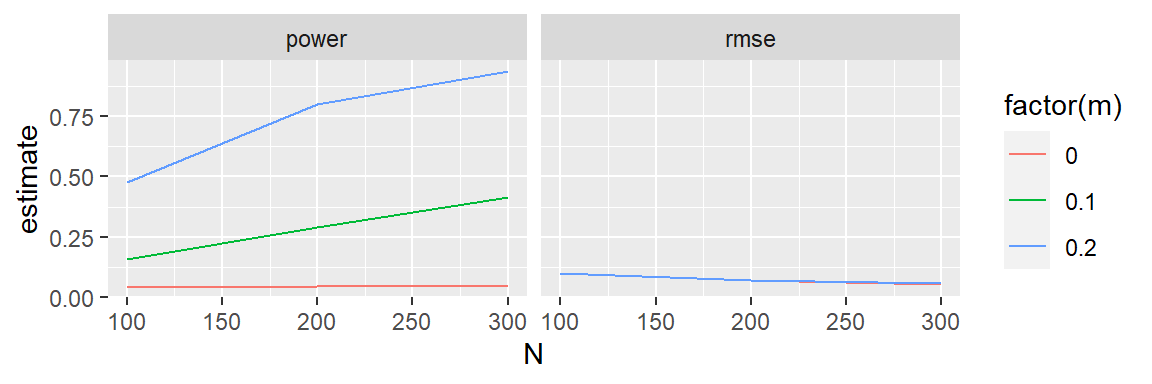
\includegraphics[width=0.5\textwidth,height=\textheight]{3.2_bayes_files/figure-beamer/unnamed-chunk-53-1.pdf}

}

\end{figure}
\end{frame}

\begin{frame}{Posterior on a quantity of interest}
\protect\hypertarget{posterior-on-a-quantity-of-interest-1}{}
What is the probability of observing \emph{strategic} first round
cooperation?

A player with rationality \(r_i\) will cooperate strategically with
probability \(r_i\) if \(r_i<.5\) and 0 otherwise. Thus we are
interested in \(\int_0^{.5}r_i/\theta dr_i = .125/\theta\)

\begin{figure}

{\centering \includegraphics[width=0.5\textwidth,height=\textheight]{3.2_bayes_files/figure-beamer/unnamed-chunk-54-1.pdf}

}

\end{figure}
\end{frame}



\end{document}
